%% Begin slides template file
\documentclass[11pt,t,usepdftitle=false,aspectratio=169]{beamer}
%% ------------------------------------------------------------------
%% - aspectratio=43: Set paper aspect ratio to 4:3.
%% - aspectratio=169: Set paper aspect ratio to 16:9.
%% ------------------------------------------------------------------

\usetheme[nototalframenumber,foot,logo]{uibk}
%% ------------------------------------------------------------------
%% - foot: 	Add a footer line for conference name and date.
%% - logo: Add the university logo in the footer (only if 'foot' set).
%% - bigfoot/sasquatch: Larger font size in footer.
%% - nototalslidenumber: Hide the total number of slides (only if 'foot' set)
%% - license: Add CC-BY license symbol to title slide (e.g., for conference uploads)
%%   (TODO: At the moment no other licenses are supported.)
%% - licenseall: Add CC-BY license symbol to all subsequent slides slides
%% - url: use \url{} rather than \href{} on the title page
%% - nosectiontitlepage: switches off the behaviour of inserting the
%%   titlepage every time a \section is called. This makes it possible to
%%   use more than one section + thanks page and a ToC off by default.
%%   If the 'nosectiontitlepage' is set you can create UIBK title slides
%%   using the command '\uibktitlepage{}' in your document to create
%%   one or multiple title slides.
%% ------------------------------------------------------------------

%% ------------------------------------------------------------------
%% The official corporate colors of the university are predefined and
%% can be used for e.g., highlighting something. Simply use
%% \color{uibkorange} or \begin{color}{uibkorange} ... \end{color}
%% Defined colors are:
%% - uibkblue, uibkbluel, uibkorange, uibkorangel, uibkgray, uibkgraym, uibkgrayl
%% The frametitle color can be easily adjusted e.g., to black with
%% \setbeamercolor{titlelike}{fg=black}
%% ------------------------------------------------------------------

%\setbeamercolor{verbcolor}{fg=uibkorange}
%% ------------------------------------------------------------------
%% Setting a highlight color for verbatim output such as from
%% the commands \pkg, \email, \file, \dataset 
%% ------------------------------------------------------------------


%% information for the title page ('short title' is the pdf-title that is shown in viewer's titlebar)
\title[TheObservatory]{Distributed Systems Project}
\subtitle{TheObservatory}


\author[Fabio Plunser \& Dominik Barbist \& Florian Gruber]{Fabio Plunser, Dominik Barbist, Florian Gruber}
%('short author' is the pdf-metadata Author)
%% If multiple authors are required and the font size is too large you
%% can overrule the font size of author and url by calling:
%\setbeamerfont{author}{size*={10pt}{10pt},series=\mdseries}
%\setbeamerfont{url}{size*={10pt}{10pt},series=\mdseries}
%\URL{}
%\subtitle{}

\footertext{{\LaTeX} beamer theme}
\date{2017-07-25}

\headerimage{3}
%% ------------------------------------------------------------------
%% The theme offers four different header images based on the
%% corporate design of the university of innsbruck. Currently
%% 1, 2, 3 and 4 is allowed as input to \headerimage{...}. Default
%% or fallback is '1'.
%% ------------------------------------------------------------------

\begin{document}

%% ALTERNATIVE TITLEPAGE
%% The next block is how you add a titlepage with the 'nosectiontitlepage' option, which switches off
%% the default behavior of creating a titlepage every time a \section{} is defined.
%% Then you can use \section{} as it's originally intended, including a table of contents.
% \usebackgroundtemplate{\includegraphics[width=\paperwidth,height=\paperheight]{titlebackground.pdf}}
% \begin{frame}[plain]
%     \titlepage
% \end{frame}
% \addtocounter{framenumber}{-1}
% \usebackgroundtemplate{}

%% Table of Contents, if wanted:
%% this requires the 'nosectiontitlepage' option and setting \section{}'s as you want them to appear here.
%% Subsections and subordinates are suppressed in the .sty at the moment, search
%% for \setbeamertemplate{subsection} and replace the empty {} with whatever you want.
%% Although it's probably too much for a presentation, maybe for a lecture.
%% Please note: \maketitle allows you to render a uibk-style title page wherever needed
%% in the document even if 'nosectiontitlepage' option is set (note: \maketitle will not
%% create a new section and is therefore not included in \tableofcontents (if used).
% \maketitle
% \begin{frame}
%     \vspace*{1cm plus 1fil}
%     \tableofcontents
%     \vspace*{0cm plus 1fil}
% \end{frame}


%% this sets the first PDF bookmark and triggers generation of the title page
\section{The Observatory}

%% this just generates PDF bookmarks
\subsection{Overview}

%% first slide
\begin{frame}
	\frametitle{Overview}


	\bigskip
	\begin{enumerate}
		\item {System architecture}
		\item {Datasets, Models, Tools \& Frameworks}
		\item {Live demo}
		\item {Evaluation results}
	\end{enumerate}

\end{frame}

%% this just generates PDF bookmarks
\subsection{System architecture}

%% first slide
\begin{frame}
	\frametitle{System architecture}
	\begin{enumerate}
		\item IoT layer provides video sources and handles alarms (ESP32-CAM, webcams, alarms, etc.)
		\item RTSP Server running on edge
		\item Edge server handles real-time detection and tracking, also auto discovery for iot devices MDNs
		\item Nast server for messaging between edge and cloud
		\item Cloud services (AWS S3, Rekognition) manage storage and face matching
	\end{enumerate}
\end{frame}

\begin{frame}
	\frametitle{System architecture}
	\vspace{1cm}
	\begin{figure}
		\centering
		
\includegraphics{_images/Distributed_Systems_Architecture_V2.png}
	\end{figure}
\end{frame}

%% this just generates PDF bookmarks
\subsection{Datasets, Tools \& Frameworks}

%% first slide
\begin{frame}
	\frametitle{Datasets, Models, Tools \& Frameworks}
	\begin{itemize}
		\item Datasets: WiseNet for surveillance scenarios
		\item Models:
		      \begin{itemize}
			      \item YOLOv8n-face with ByteTrack for multi object face detection
			      \item Mobilenet\_v3\_small for REID implementation
		      \end{itemize}
		\item Tools: FFmpeg, OpenCV, RTSP, NATS, SQLite,
		\item Frameworks: 
		\begin{itemize}
			\item PyTorch 
			\item FastAPI
			\item Docker
			\item Svelte  
		\end{itemize}
	\end{itemize}
\end{frame}

%% this just generates PDF bookmarks
\subsection{Live Demo}

%% first slide
\begin{frame}
	\frametitle{Live Demo}
	\begin{itemize}
		\item Automatic connection Iot to edge server
		\item Real-time detection of faces on incoming video streams
		\item Automatic alarm trigger upon unknown face detection
		\item Web-based dashboard for live status updates
	\end{itemize}
\end{frame}

%% this just generates PDF bookmarks
\subsection{Evaluation Results}

%% first slide
\begin{frame}
	\frametitle{Evaluation Results}
	\begin{itemize}
		\item Parallel stream handling performance measured at different loads
		\item Scalable but requires GPU resources for higher frame rates
		\item Measured resource usage (GPU/CPU) at various parallel processing levels
		\item Measured average 15 fps with 6 parallel cameras
		\item Detect unknown face in under 2 seconds (average)
		\item Cloud requests remain under 1s on average
		\item $\approx$ 20\% of uploaded face images do not contain a face
	\end{itemize}
\end{frame}

\begin{frame}
\frametitle{Additional Metrics}
\begin{itemize}
	\item Frame skip rate: 25\% at high loads (over 8 cameras)
	\item GPU usage: up to 80\% on NVIDIA RTX 3080 for detection
	\item CPU usage: 40\% average on 12-core AMD Ryzen 9
	\item Memory usage: 12GB average with 6 camera feeds
\end{itemize}
\end{frame}
\begin{frame}
	\frametitle{Additional Metrics}
	\begin{figure}
		\centering
		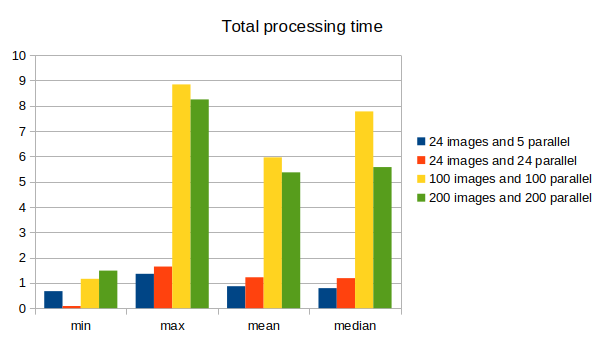
\includegraphics[width=0.80\linewidth]{_images/total_processing_time.png}
	\end{figure}
\end{frame}
%% to show a last slide similar to the title slide: information for the last page
\title[TheObservatory]{Distributed Systems Project}
\subtitle{TheObservatory}
\section{Thanks}

\end{document}
